\documentclass[a4paper,10pt]{article}

\usepackage[utf8]{inputenc}
\usepackage[T1]{fontenc}
\usepackage[danish]{babel}

\usepackage{color}
\usepackage{float}
\usepackage{fancyvrb}

\usepackage{amssymb}
\usepackage{amsmath}
\usepackage{listings}
\usepackage{comment} 
\usepackage{hyperref}
\usepackage{bookmark}

\usepackage{graphicx}
\usepackage[]{algorithm2e}
\def \hitchars {\{\{\text{a}:?...\text{z}:?\},\{\text{A}:?...\text{Z}:?\}...\}}

\DeclareGraphicsExtensions{.png}

\definecolor{dkgreen}{rgb}{0,0.45,0}
\definecolor{gray}{rgb}{0.5,0.5,0.5}
\definecolor{mauve}{rgb}{0.30,0,0.30}

% Default settings for code listings
% Default settings for code listings
\lstset{frame=tb,
  language=Java,
  aboveskip=3mm,
  belowskip=3mm,
  showstringspaces=false,
  columns=flexible,
  basicstyle={\small\ttfamily},
  numbers=left,
  numberstyle=\footnotesize,
  keywordstyle=\color{dkgreen}\bfseries,
  commentstyle=\color{dkgreen},
  stringstyle=\color{mauve},
  frame=single,
  breaklines=true,
  breakatwhitespace=false
  tabsize=1
}

%indsætjeres navn herunder.
\title{Introduction to Programming - Re-exam Project (Part I) \\\rule{10cm}{0.5mm}}
\author{Simon Dradrach Jørgensen 
\\Supervisor: Peter Schneider Kamp \\ DM550 \\\rule{5.5cm}{0.5mm}\\}
\date{\today}

\begin{document}

\maketitle

\vfill

\tableofcontents
%laver forside og indholsfortegnelse

\newpage

\section{Specification} 
%forklar hvad programmet skal gøre

The given task is to write a program in \textit{Python}, that encrypts a message, based on the \textbf{Caesar-cipher}, which is used in \textbf{cryptography}.
The way it works is, a person is given a \textbf{plain text} to encrypt into a coded message, this is done by shifting the letters in the message, by a value of \textit{n}, e.g., 

\textit{shifting w by 6: w $\rightarrow x \rightarrow y \rightarrow z \rightarrow a \rightarrow b \rightarrow c$ (result is  c)}.

There's in-built functions in python that can come up with a needed result, rather easily aswell. However, knowledge of the required key is a great threat for the \textit{encrypted} message, it'd become too easy to decipher, and serve no purpose. 

With that goal in mind, one can quickly figure out that it's not safe to have a program with a given key to encrypt the message, since the key is known. The second task brings that issue to mind, where an encrypted message is given, without a known key. Here one is supposed to find a way to find the desired key to decrypt the message.

The program should be able to support multiple \textit{sets} of symbols. To help create the range of symbols, a function must be designed, such as the function is capable of receiving a starting entry and an end entry. The starting entry will in this case be the first \textit{character} in both \textit{lists} of the two-dimensional \textit{list}, and the end entry will be the last \textit{character} in the \textit{lists}.

\section{Design}
%hvordan projektet blev planlagt, hvilke tanker gik ind i hvordan problemet skulle løses

\subsection{Part 1}

If one could use the key to to shift through the \textit{characters} in the message given, the task can be completed in a rather simple way; with the useage of \textbf{integers}. Python can convert \textit{characters} to integers, with the \textbf{ord()} in-built function. This makes one capable in shifting through the desired \textit{n}-value of shifts, to encrypt a message, and to convert the integers back to \textit{characters}, Python has another in-built function, the \textbf{chr()}, which converts the integers back to \textit{characters}.
As one would think, the way to decrypt an encrypted message, is simply to do the shifts backwards, meaning, instead of doing \textit{n} shifts, one would have to do \textit{-n} shifts.

The problem with using \textbf{ord()} and \textbf{chr()} however, is that they represent the \textit{alphabet} in a \textit{homogenize} way, since there's an unnecessary space between the small and capital letters.
Instead of converting \textit{characters} into integers, they can be indexed in a \textit{set}, e.g., \{0 : a, 1 : b, 2 : c, 3 : d, 4 : e\}.
Because shifting from small to capital letters would be unwise, these sets are to be two-dimensional, e.g., 

\{\{0 : a, 1 : b, 2 : c, 3 : d, 4 : e\}, \{0 : A, 1 : B, 2 : C, 3 : D, 4 : E\}\}.

\subsection{Part 2}

The specification requires a \textit{histogram class}, this class requires two different constructors, these constructors are to differentiate between a \textbf{.dat} file, and a \textbf{.crypt} files. The first constructor, is to load each \textit{character}, with its own occurence and the second constructor is to account each occurence for every occuring \textit{character}. During the counting, the constructor is to filter symbols not inside the two-dimensional list.
The class is also to own a function to create a list, this list is to be sorting with the keys, being the occurence of every symbol, descending. A final function must be implemented to enable statistical abbreviation of the key, using the list of two different \textit{histograms}.

The way \textit{histogram} works in the following task, is by using the \textbf{.dat} file, to construct \textit{frequencies}\cite{1}:

\begin{figure}[htp]
\centerline{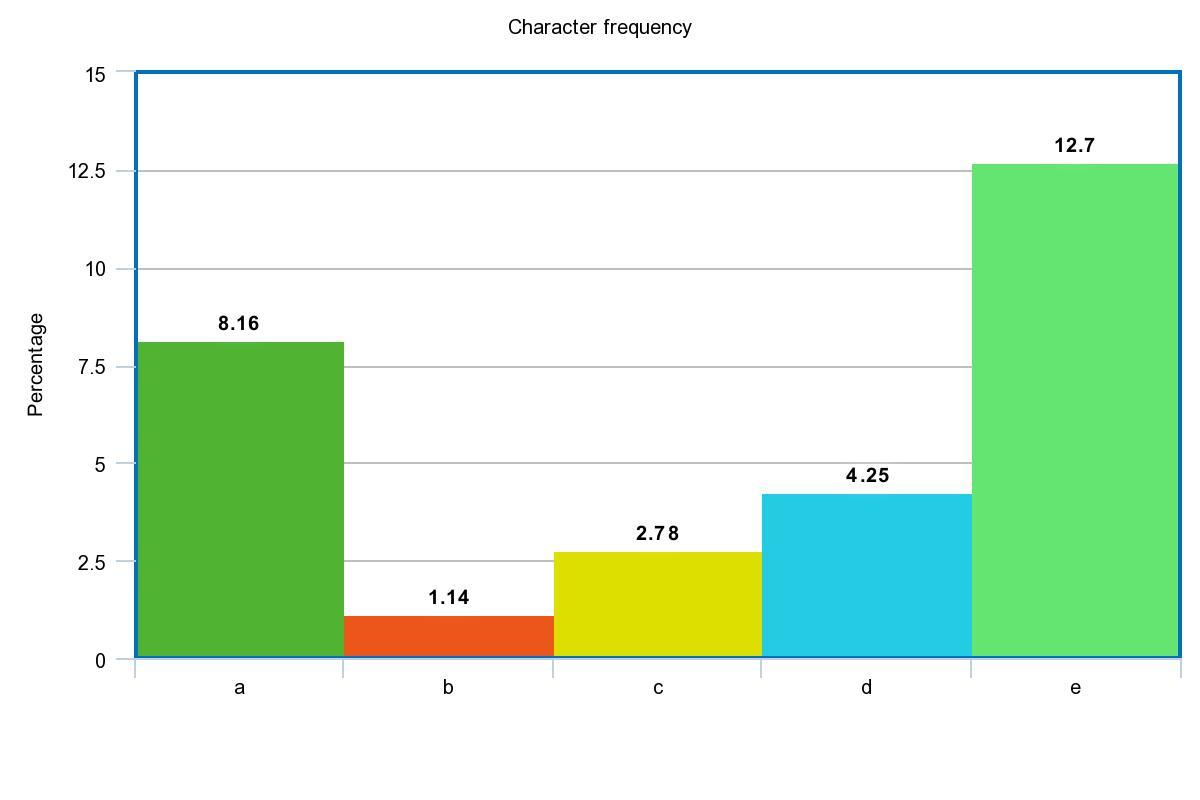
\includegraphics[width=15cm]{meta-chart.jpeg}}
\caption{Histogram}
\label{fig:meta-chart.jpeg}
\end{figure}

These \textit{frequencies} were used to plot the overall occurences of a given \textit{character} in the \textit{lists} within the \textit{dictionary}.

\section{Implementation}
%hvordan skrev du programmet
%forklar hvordan delene af dit program virker

\subsection{Part 1}

Due to the requirements of the \textit{sets}, a function for creating a range of the symbols that are to be rotated, must be implemented. The way the rotations work, is the following example:

\begin{itemize}
    \item $\{a, b, ... , x, z,\rightarrow , a, b\}$
\end{itemize}

The reasoning for this requirement, is because of the \textbf{ord()} function converting the  \textit{characters} into \textbf{unicode}, which are essentially \textit{integers}, e.g.,

\begin{lstlisting}[language=python]
print(ord('a'))
\end{lstlisting}

The following result would be 97, and \textit{z} would be 122 in the row. However, if one would shift an additional time, one would get the symbol, "\{", therefore it's important to have a \textit{set} range between \textit{a} and \textit{z}, and when the shift is made from \textit{z}, the list would rotate back from the start. The exact same idea is used for capital letters.

To convert the \textit{integers} back to \textit{characters}, one must simply use the reverse function of \textbf{ord()}, with the in-built function \textbf{chr()}:

\begin{lstlisting}[language=python]
print(chr(97))
\end{lstlisting}

This will result in: \textit{a}, which is the inverse of the already implemented \textbf{ord()} function. With these in-built functions from the python library, it's possible to convert a given \textit{character} into its \textit{integer} representation, and shift with that, before converting back to the \textit{character} representation of the now shifted \textit{integer}.

\begin{lstlisting}[language=python]
def srange(s, e = None, step = 1 ,sj = 0, ej = 0):
    r = range(ord(s) + sj, ord(e) + ej, step) if e else range(0, ord(s) + sj, step)
    return [chr(x) for x in r]
\end{lstlisting}

Since Python already has an in-built range-function, taking inspiration from that function, would be the most ideal solution for the arguments.
However, due to Python's inability to increment \textit{characters}, two arguments for incrementing the \textit{characters} must be implemented to increment the \textit{characters}, hereby the origin of the \textit{sj (start-jump)}, and \textit{ej (end-jump)}.


When creating the cipher, one must realize that the \textit{sets} of \textit{characters} that are to be rotated, is a two-dimensional list, hereby allowing for each list inside the two-dimensional list, to be rotated individually. Due to the fact, that the most idiomatic way is to replace \textit{characters} in a string, is via a dictionary, one must create a dictionary for each list in the two-dimensional list, and \textit{merge} the created dictionaries to obtain one complete dictionary, to be later used in the in-built \textit{string-translate} function.

To do this, two functions must be created locally inside the cypher-function, these functions are the \textit{table} and \textit{merge} functions.

\begin{lstlisting}[language=python]
def cypher(key, message):
    def table(l):
        ...
    def merge(l):
        ...
\end{lstlisting}

The \textit{table} function creates a dictionary, with the keys being an integer representation of each of the elements in the list, and the value be each of the rotated elements in the list. This setup fits the arguments of the in-built \textit{string-translate} function. The \textit{merge} function will run \textit{n} times, depending on the length of the first dimension in the two-dimensional list, with each arguments being the output of a new \textbf{iteration}, of the \textit{table} function. Thus the in-built \textit{string-translate} function will use the \textit{merged} dictionary to rotate all necessary \textit{characters}.

\newpage

\subsection{Part 2}

In python for a class to have multiple constructors, the useage of the \underline{@staticmethod} \textit{wrapper-class} is required. Since \underline{@staticmethod} creates a non-member static function, it gives the idea of non-preference, since in multiple languages, static methods are not allowed to change the input \textit{parameters}. Because the function to compare the two lists from the \textit{histograms} has no preference, and the lists are not a variable in the \textit{histogram} themselves.

The function for loading \textit{.dat}-file aptly named \textit{key}, takes every line in the given \textit{string} and uses the first \textit{sub-string} as the key, and the second \textit{sub-string} as the value. Afterwards, calls the \textit{histogram's} default constructor with a list of \textit{dictionaries} and a \textit{boolean}, which tells the constructor whether or not it should \underline{fractor} the given list of \textit{dictionaries}. However, to load a sample file, the \textit{key} function, needs some help, an example for this, could be:

\begin{lstlisting}[language=python]
eng = histogram.key((filter(lambda s: len(s), x.split(" ")) for x in f))
\end{lstlisting}

The function for loading a \textit{.crypt} file, aptly named \textit{text}, counts every occurrence, for every character occurring in the given \textit{string}.

The default constructor for the \textit{histogram} class, allows for \textit{fracturing} of the given lists of \textit{dictionaries}. \textit{Fracturing} follows the following \textbf{Pseudo-code}:

\begin{algorithm}[H]
 \For{$d \in \hitchars$}{
    $s:=\sum\limits_{i=0}^{|d|-1}{(d_i)_1}$ \;
    \For{$v \in d$}{
        $v_1 \leftarrow \dfrac{v_1}{s}$ \;        
    }

 }
\end{algorithm}

This algorithm replaces each keys absolute occurrence, with relational occurrence, compared to the sum of all occurrences.

As the specification demands, the \textit{histogram} class is to have a function, capable of creating a sorted \textit{list} from the \textit{histogram} itself. This is done by converting the \textit{dictionary} in the \textit{histogram} into a list, and sorting every element in the \textit{list} depending on the value of the key.

\begin{algorithm}[H]
 \For{$d \in \hitchars$}{
    $d \leftarrow \{e_0 | e \in sort \ d \}$
 }
\end{algorithm}

To calculate the desired key, one initially calculates a list of the distances between each element with the following function: $f(a,b) = (b-a) \ mod \ 26$. The most occuring element is then chosen as the key.

\newpage

\section{Testing}

In the testing phase of part 1, a simple logical mindset was used, converting a \textit{string} into an \textit{integer}, and then adding an \textit{n}-value to it, before converting it back to a \textit{string}. Then printing the \textit{string} to check if the characters had shifted towards the desired value.

Part 2 was a bit tricky, due to the fact that a \textit{dictionary} does not add elements in a predictable order, thus an ordered \textit{dictionary} was required for this task. A number of statistical functions were also used, however, the function that returned the most occurring element proved to be the most proficient function.

To launch the program, one must use the following command:

\subsection{Part 1}
\begin{lstlisting}[language=command.com]
$ python3 caesar.py ( N ) < hello.txt > result.txt
\end{lstlisting}

Where N is the value of the shifts, that the program will perform before saving the file at the desired location, with the given result after the shift.

\subsection{Part 2}
\begin{lstlisting}
$ python3 histogram.py engelsk.dat < engelsk1.crypt.txt > result.txt
\end{lstlisting}

Where the program will read the encrypted \textbf{.crypt} file, and save the decrypted \textbf{.txt} file in the desired location.

\begin{comment}
I testing skal i forklare jeres tests osv. udover det kan i have et billede med
som i kan tilføje ved at kopiere includegraphics som herunder.

\begin{figure}[H]\center
\includegraphics[scale=1]{billede.png}
\caption{}
\end{figure}

udskift billede.png med jeres billede fil som skal ligge i samme mappe som .tex
i kan ændre på scale for at ændre pÃ¥ billede størrelse i pdfen.
\end{comment}

\section{Conclusion}
%hvad kom i frem til, gik noget galt? kunne noget gøres bedre?
To conclude the project, the useage of \textit{dictionaries} in python, is to be respected, since the order of inserted elements is \textbf{inhomogeneous}.
Sadly, only 2 out of 3 \textbf{.crypt} files were solved, namely: \textbf{engelsk1.crypt.txt} and \textbf{engelsk3.crypt.txt}. The file that couldn't be solved had too many distances with equal or almost equal occurrences.
This can point towards, that the program might not be perfect to solve the required task, even if it did solve 2 out of 3 tasks.

The \textbf{python3 interpreter} is required to launch the program, due to the useage of the \textit{system} library, e.g.,

\begin{lstlisting}[language=python]
print(cypher(args.key, sys.stdin.read()))
\end{lstlisting}

\newpage

\section{Appendix (source code)}
%lstinputlisting tilføjer jeres sourcecode, jeres python fil skal bare ligge i samme mappe som .tex filen husk at fjerne %

\subsection{Part 1}

\begin{lstlisting}[language=python]
def srange(s, e = None, step = 1 ,sj = 0, ej = 0):
    #[s+sj;e+ej;step[
    r = range(ord(s) + sj, ord(e) + ej, step) if e else range(0, ord(s) + sj, step)
    return [chr(x) for x in r]
#s = start
#sj = start jump
#e = end
#ej = end jump

hitchars = [srange("a", "z", ej = 1), srange("A", "Z", ej = 1)]
#[a;z+1[, Range of all lowercase characters
#[A;Z+1[, Range of all uppercase characters

def cypher(n, s, tables = hitchars):
    def table(l):
        return {ord(x) : y for x, y in
                    zip(l, l[n:] + l[:n])}

        #l = Original l (list)
        #l[n:] + l[:n] = Rotated l (list)

    def merge(l):
        i = iter(l)
        #create iterator for l (list).
        z = next(i).copy()
        #get the first element from the iterator and copy it
        for x in i:
            #get the remaining elements
            z.update(x)
            #Update the copied element(z) with the remaining elements in the iterator

        return z

    s = s.translate(merge((table(l) for l in tables)))
    return s

def decypher(n, s, tables = hitchars):
    return cypher(-n, s, tables)

if __name__ == "__main__":
    import argparse, sys
    parser = argparse.ArgumentParser(description='Run a ceasar cypher.')
    parser.add_argument('key', metavar = 'N', type = int, help = 'The key for shifting the charaters')
    args = parser.parse_args()
    print(cypher(args.key, sys.stdin.read()))
\end{lstlisting}
\newpage
\subsection{Part 2}
\begin{lstlisting}[language=python]
from operator import itemgetter
import collections
from collections import OrderedDict
from caesar import hitchars, decypher

def find(c, ll):
    for i, l in enumerate(ll):
        if c in l:
            return i
    return -1

class histogram:
    def __init__(self, ld, frac=False):
        if frac:
            self.stat = ld
            for d in self.stat:
                s = sum(d.values())
                for k in d:
                    d[k] = d[k]/s
        else:
            self.stat = ld

    def list(self):
        def f(d):
            return [e[0] for e in sorted(d.items(), key = itemgetter(1), reverse = True)]
        return [f(d) for d in self.stat if d]

    @staticmethod
    def compare(a, b):
        #Estimate shift.
        def dist(x, y, n):
            return ((hitchars[n].index(y) - hitchars[n].index(x)))%len(hitchars[n])
        def mode(l):
            return collections.Counter(l).most_common(1)[0]


        d = [dist(x, y, i) for i, ll in enumerate(zip(a,b)) for x, y in zip(ll[0], ll[1])]
        return mode(d)[0]

    @staticmethod
    def text(s, frac=False):
        #to be used as a constructor
        #creates a histogram from a text
        ld = [OrderedDict() for x in hitchars]
        for c in s:
            n = find(c, hitchars)
            if n >= 0:
                ld[n][c] = ld[n].get(c, 0) + 1
        return histogram(ld, frac)

    @staticmethod
    def key(s, frac=False):
        #to be used as a constructor
        #creates a histogram from a list of element and occurences
        ld = [OrderedDict() for x in hitchars]
        for c, v in s:
            n = find(c, hitchars)
            if n >= 0:
                ld[n][c] = float(v)
        return histogram(ld, frac)

    def __repr__(self, digits=3):
        return repr([{k : round(d[k], digits) for k in d} for d in self.stat if d])

if __name__ == "__main__":
    import sys
    with open(sys.argv[1]) as f:
        eng = histogram.key((filter(lambda s: len(s), x.split(" ")) for x in f))

    s = "".join(sys.stdin.readlines())
    t = histogram.text(s)
    print(decypher(histogram.compare(eng.list(), t.list()), s))
\end{lstlisting}

%\textbf{Sierpinski triangle program}
%\lstinputlisting[language=python]{sierpinski.py}
%\textbf{Binary tree program}
%\lstinputlisting[language=python]{binary.py}

\begin{comment}
Hvis Fern Time er lavet tilføjes det her og begin og end comment skal fjernes. 
\textbf{Fern program}
\lstinputlisting[language=python]{fern.py}

\end{comment}

\medskip
 
\begin{thebibliography}{9}
\bibitem{1}
\url{https://www.meta-chart.com/histogram}
 
\end{thebibliography}

\end{document}